\documentclass[../notes.tex]{subfiles}

\pagestyle{main}
\renewcommand{\chaptermark}[1]{\markboth{\chaptername\ \thechapter\ (#1)}{}}
\setcounter{chapter}{6}

\begin{document}




\chapter{Presentations}
\section{Day 1 (1-6)}
\begin{itemize}
    \item \marginnote{3/11:}Nate's presentation.
    \begin{itemize}
        \item Figure out what IC\textsubscript{50} means, and why nanomolar (including single-digit) is good!
        \item Explain bio terms (but I'm already planning this).
        \begin{itemize}
            \item Make sure I have oncometabolite definition right!
        \end{itemize}
        \item Make sure all mechanistic/synthetic details are right and explainable (but I'm already planning this).
        \begin{itemize}
            \item "You should be able to right a mechanism for any reaction you're going to present" - Steve.
            \item "If you're in a job interview, you have to be able to have some answer if someone asks how the reaction goes."
            \item "Sometimes I know and sometimes I don't, and then I have to look up a bunch of papers. And then sometimes I can figure it out and sometimes I can't, but at least I have something to say then." Sweet!
        \end{itemize}
    \end{itemize}
    \item Steve to Dennis: "All of these presentations should have been downloaded ahead of time."
    \item Frank's (Harvard) presentation.
    \begin{itemize}
        \item Vadadustat.
        \item "Slow down, breathe, and don't read from the slide."
        \item "You gonna walk us through that scheme? Because otherwise, it's useless."
        \begin{itemize}
            \item Make sure I explain all figures, including crystal structures!! Learn the hydrogen bonds.
        \end{itemize}
        \item Make sure I can explain ambiguous selectivity, too!!
        \item \ce{HBr} works to hydrolyze \emph{activated} (e.g., phenyl) methyl ethers (and can do nitrile hydrolysis at the same time).
        \begin{itemize}
            \item Explain selectivity for chloro S\textsubscript{N}Ar on \emph{s}-triazene vs. \emph{ortho}-pyridine.
            \item More activated/under more mild conditions. Look up typical conditions for pyridine S\textsubscript{N}Ar and look to differentiate temperature, acid, etc. from the used conditions.
        \end{itemize}
    \end{itemize}
    \item Minh's presentation.
    \begin{itemize}
        \item Voydeya.
        \item Appreciating structural/retrosynthetic challenges is probably a good idea!
        \item Make sure I know what the biuret test is (a protein test --- like the functional group tests Steve discussed that day --- that does not contain biuret, but gives a positive result to the peptide-like bonds in biuret).
        \item Check timing: Make sure I get everything in in 10 minutes, and don't linger on the bio!
        \item Sleep well both of the next two nights!
    \end{itemize}
    \item Alexander's presentation.
    \begin{figure}[h!]
        \centering
        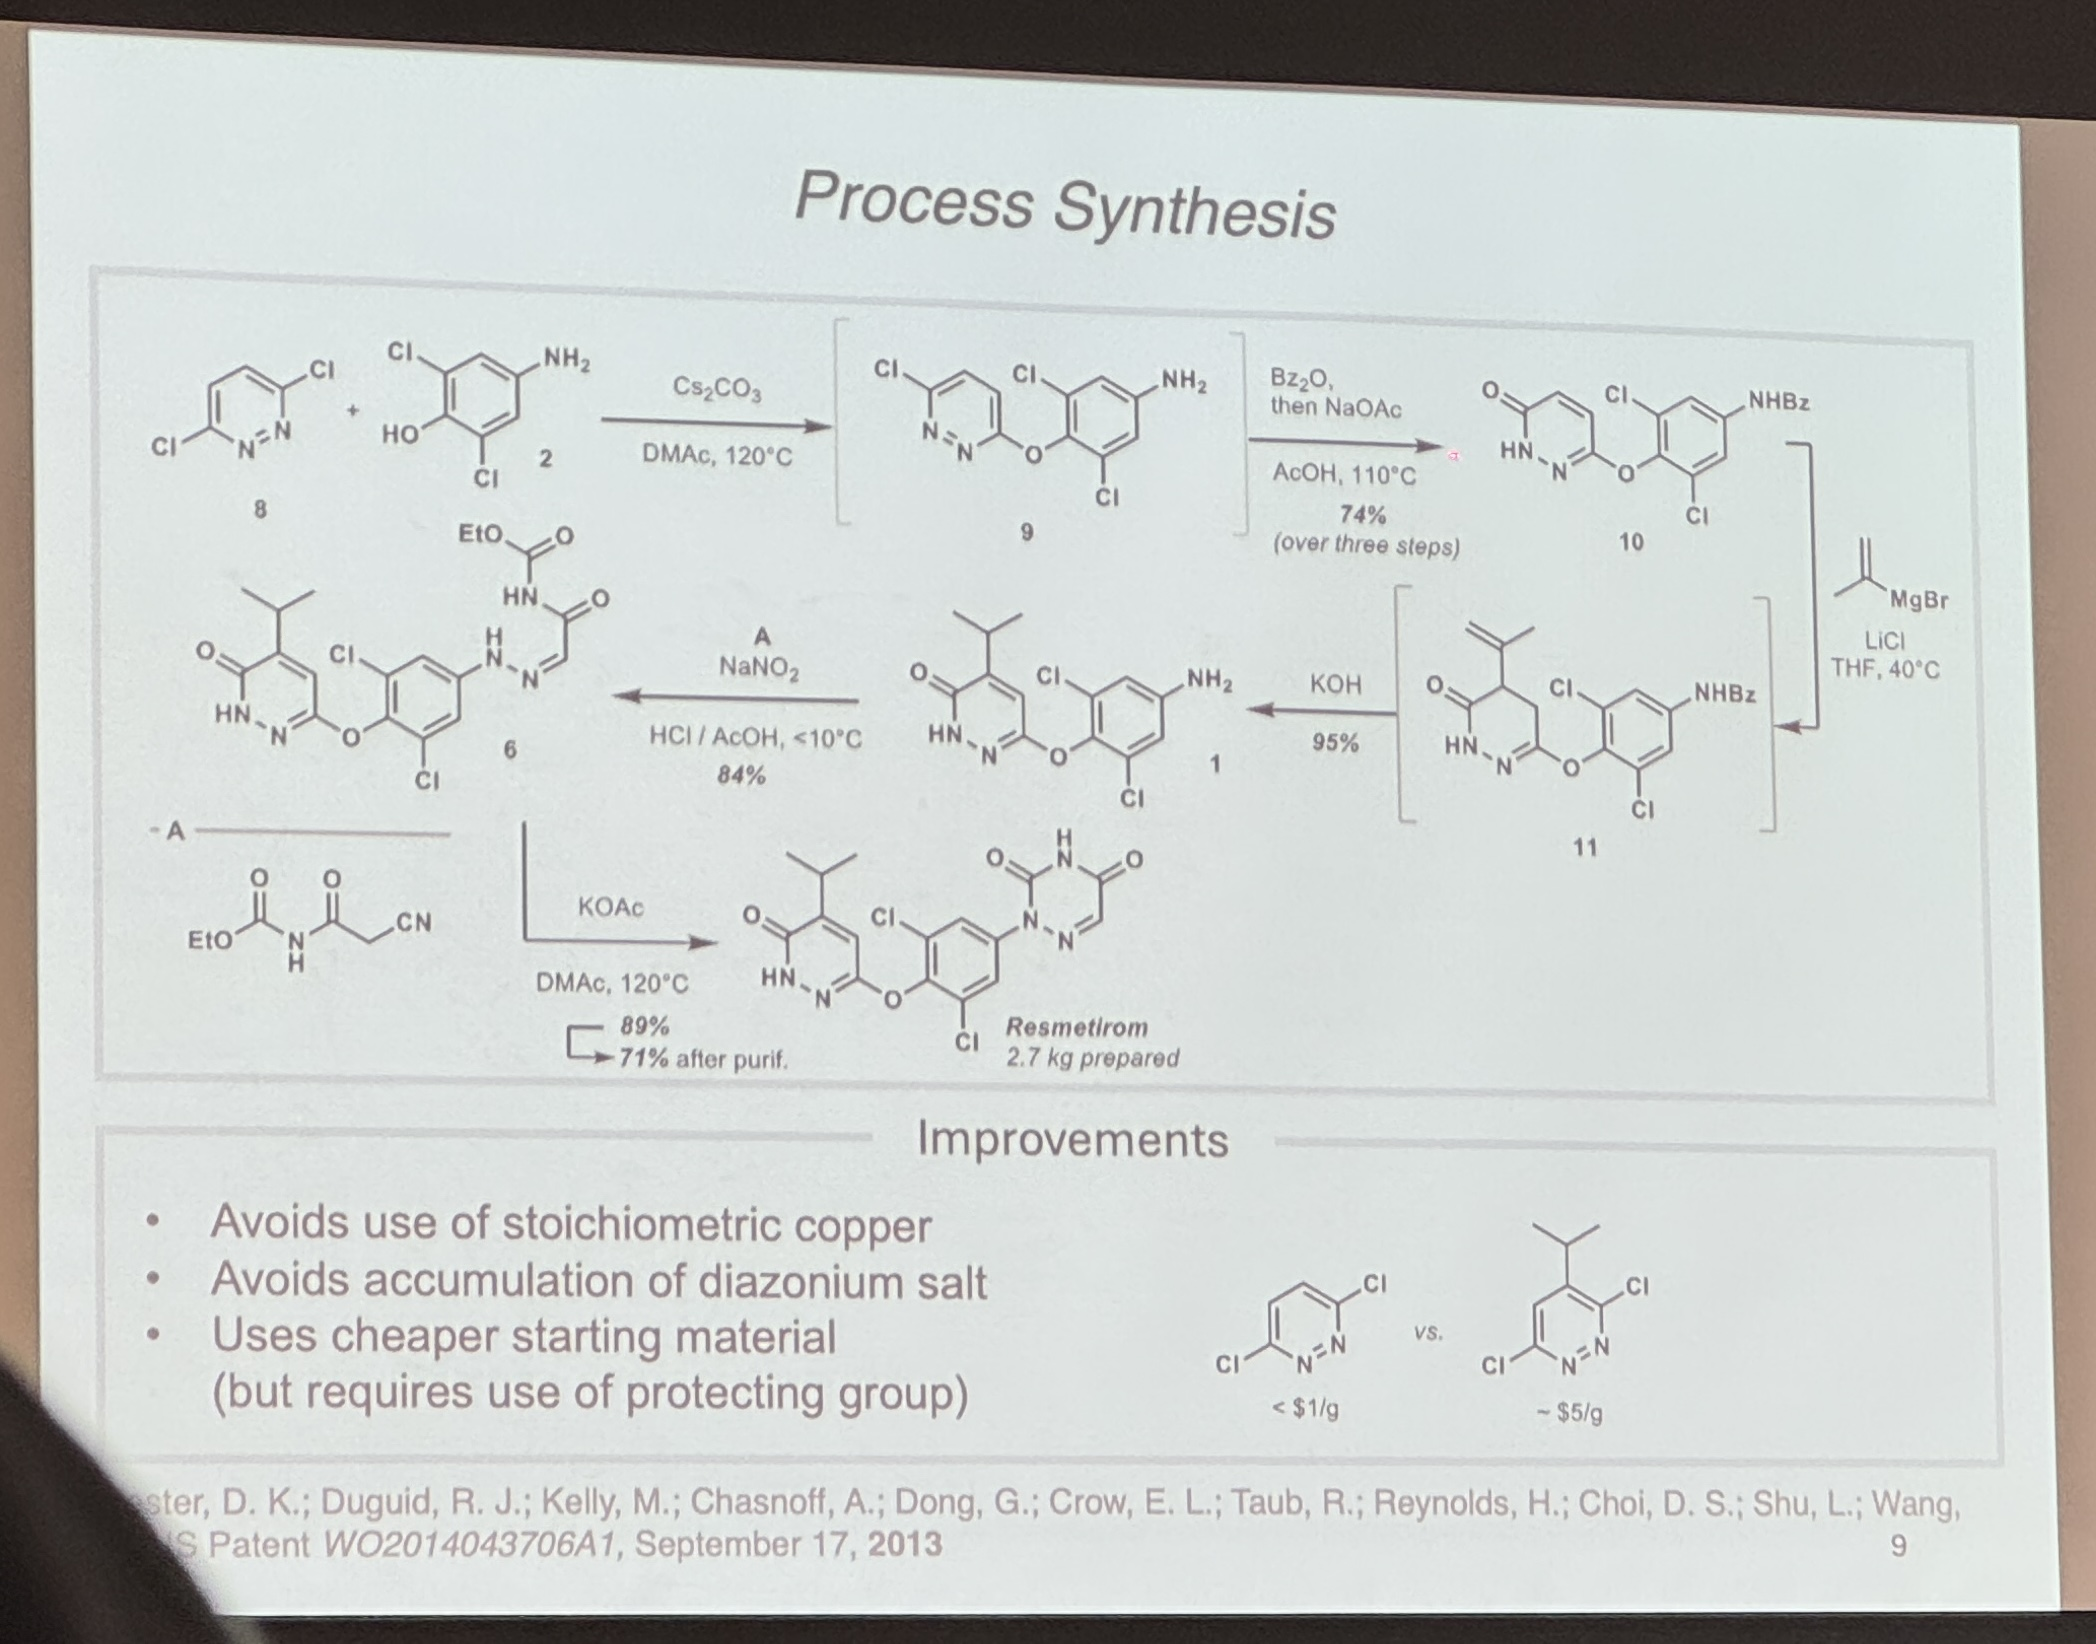
\includegraphics[width=0.7\linewidth]{PresAlexander.JPG}
        \caption{Alexander M\"{u}ller's graphic design.}
        \label{fig:PresAlexander}
    \end{figure}
    \begin{itemize}
        \item Resmetirom.
        \item Electron-rich arenes easily oxidize in the body, leading to redox cycling. Causes safety/toxidity issues.
        \begin{itemize}
            \item Good discussion of design principles; keep doing the same!
        \end{itemize}
        \item Good retrosynthesis, followed by synthesis.
        \item Dives into mechanisms of key steps.
        \item Good graphic design: Boxes. Very clean and clear. Citations in light grey at bottom left.
        \item Numbering chemicals and compounds is a good idea.
        \item Explaining selectivity is definitely needed!
    \end{itemize}
    \item Angel's presentation.
    \begin{itemize}
        \item Ceftobiprole: Staph antibiotic.
        \item Starts with retrosynthetic analysis of moieties.
        \item Gives a total nitrogen count; I could/should, too!
        \item Gives a discovery timeline.
        \item Know the mutations.
        \item Drawing out arrow-pushing mechanisms is not inappropriate.
        \item Make changes clear in large molecules moving from one to the next with colored bonds, as Steve does! Otherwise, you just get lost as to what's changing\dots
    \end{itemize}
    \item On Thursday, we'll start at 9:00 instead of 9:05.
    \item Kwanwoo's presentation.
    \begin{figure}[H]
        \centering
        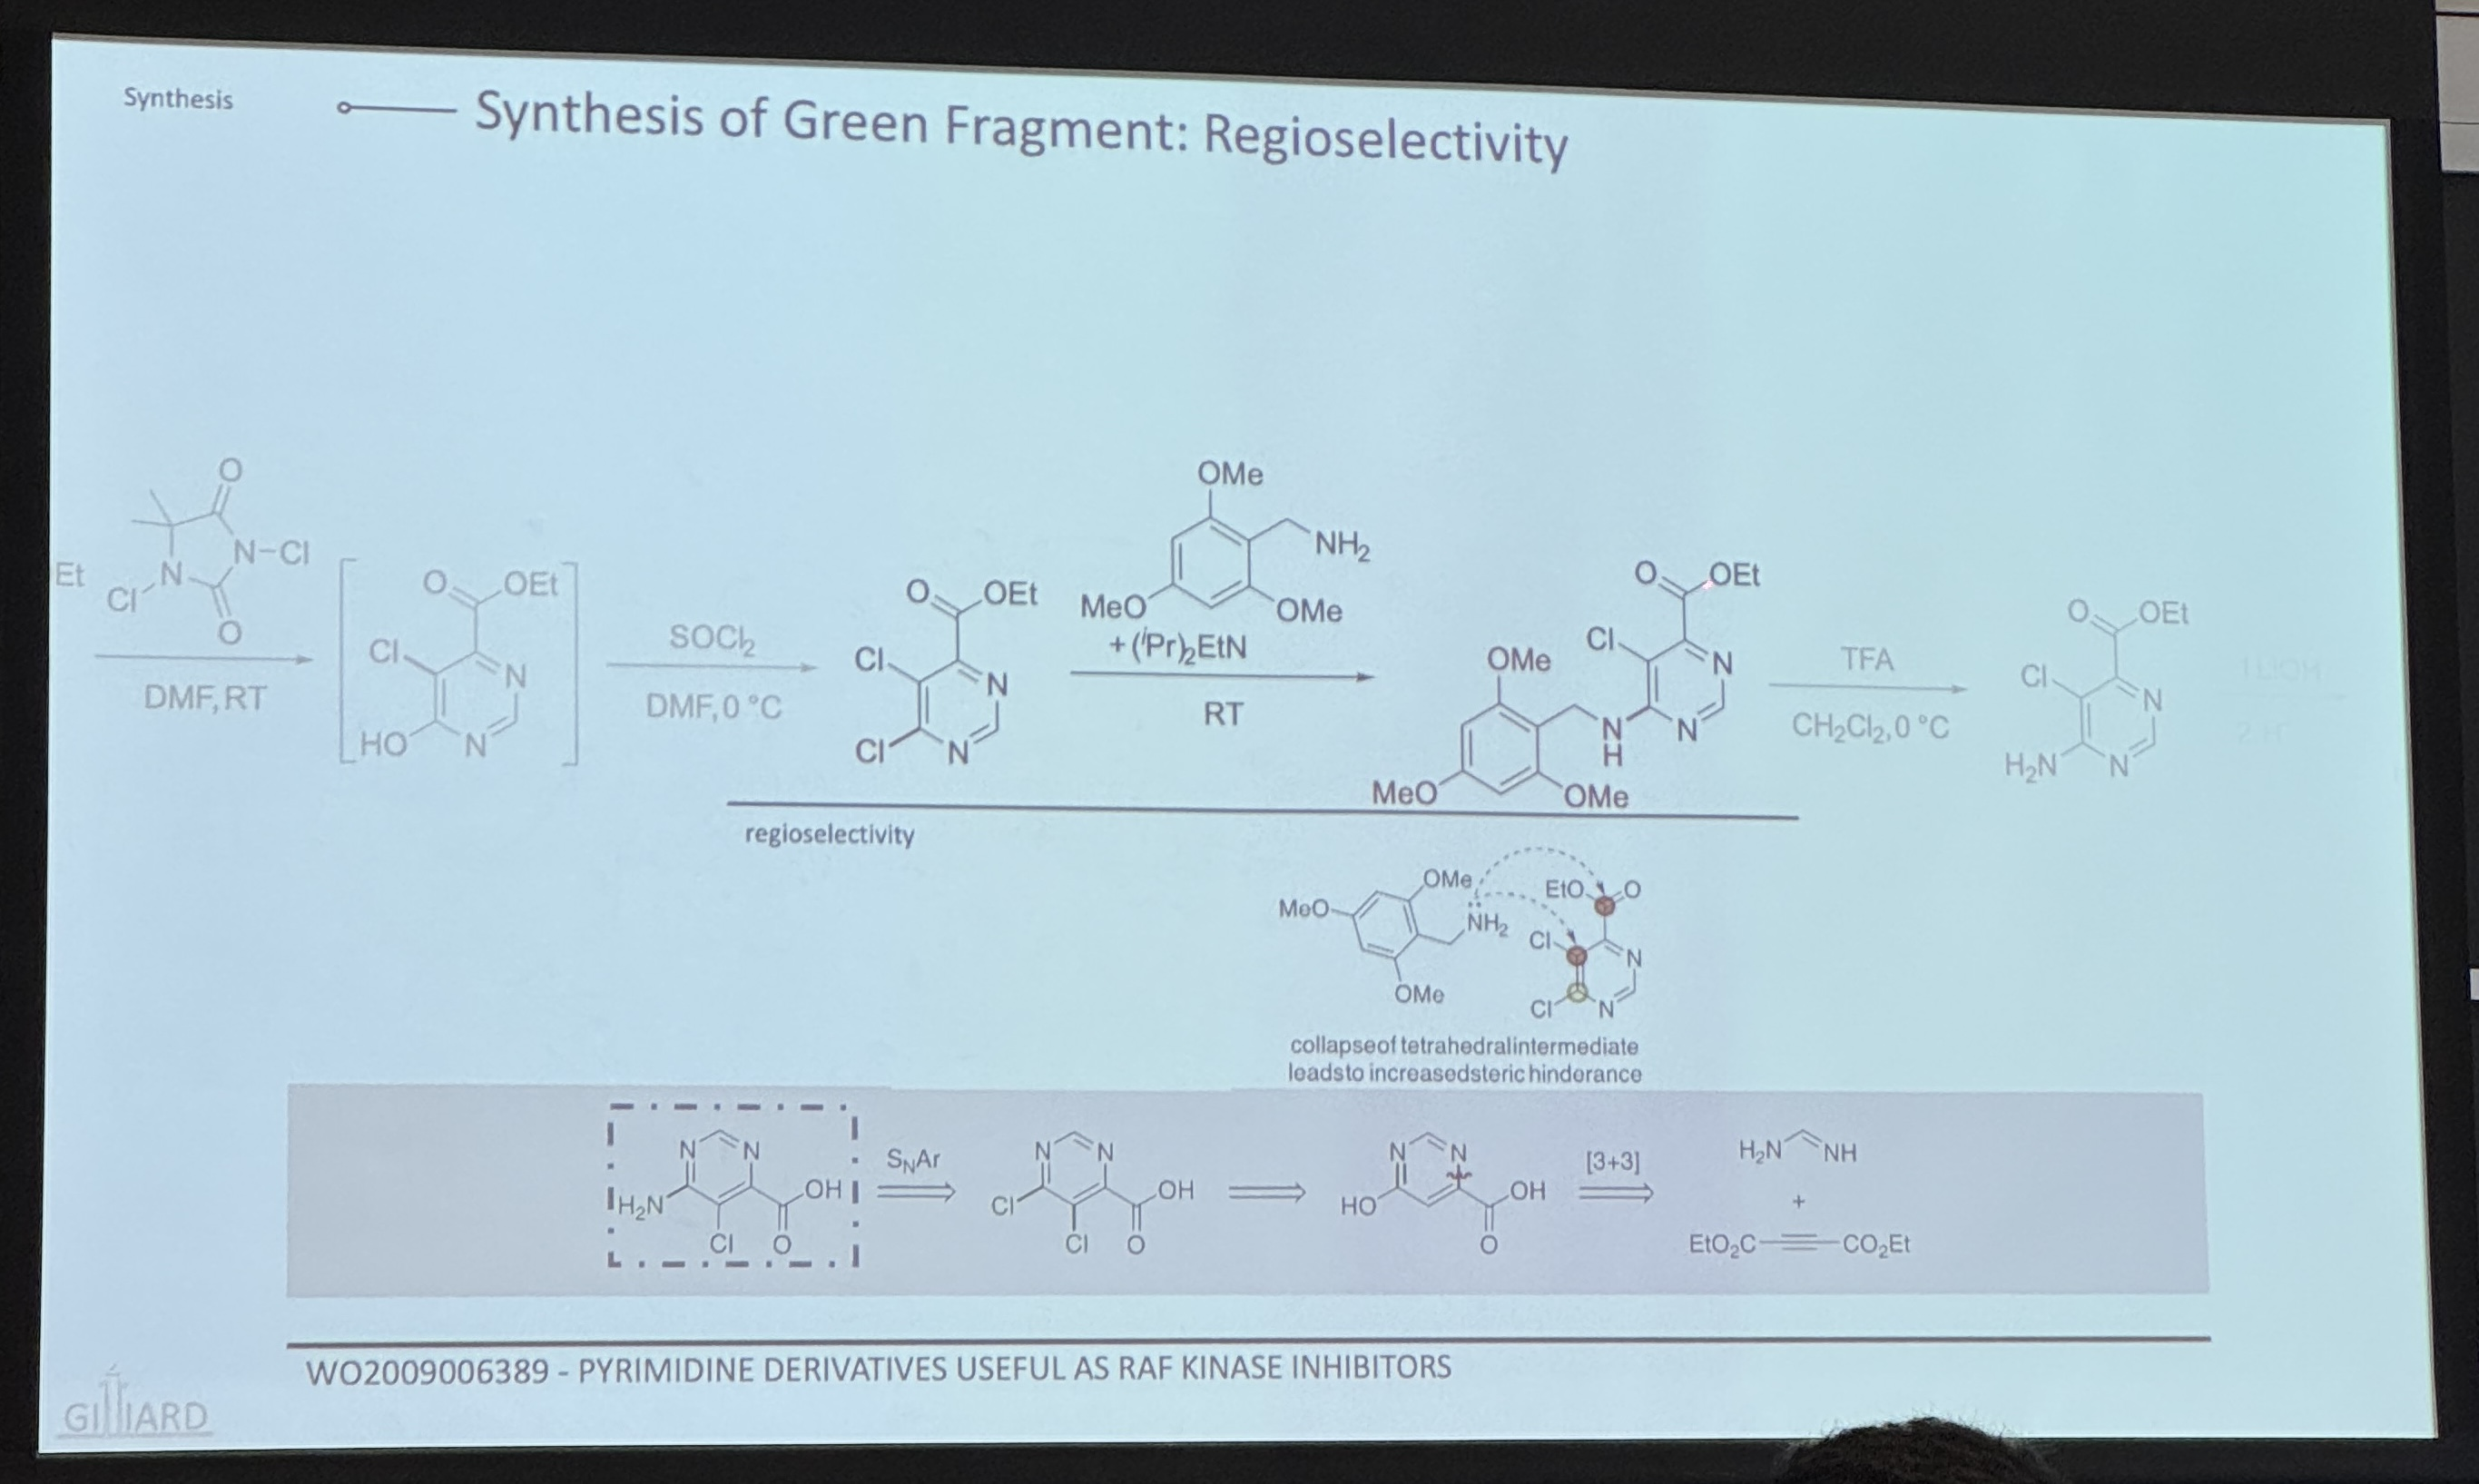
\includegraphics[width=0.7\linewidth]{PresKwanwoo.JPG}
        \caption{Kwanwoo Park's graphic design.}
        \label{fig:PresKwanwoo}
    \end{figure}
    \begin{itemize}
        \item Ojemda.
        \item Also uses MIT/Gilliard slide template!
        \item Also discussing a glioma; could give him a shoutout in my presentation!
        \item Slides are too cluttered and he's reading off the slides.
        \item Good retrosynthetic analysis. Color-codes fragments (using pastel-colored boxes might be better, then keeping them on each slide).
        \item Points out Hantzsch; I should make a fuss about names as well.
        \item Know the names of functional groups! Know the carbon numbering in my molecule.
        \item Graphic design.
        \begin{itemize}
            \item Mechanism in pop-up box is a good approach.
            \item Keeping the general scheme at the bottom of each slide, being progressively highlighted, as you move through bigger synthetic details up top.
            \item Chemoselectivity with circles in popup box.
        \end{itemize}
        \item Know reagent names, and functional group names.
    \end{itemize}
\end{itemize}




\end{document}